\chapter{Assays: Cell Adhesion Assay Validation: Tumor-Cell Adhesion to a HUVEC Monolayer}
\label{Chap:TumorCellAdhesion}

\section{Preface}
This work was performed and written in equal collaboration with Edmond Young as represents a manuscript in preparation.

\section{Introduction}
The process of cell adhesion involves physical interactions between cells and the materials in their microenvironment such as extracellular matrices, synthetic biomaterial surfaces, and other cells and is a major topic of interest in areas ranging from fundamental cell biology and pathophysiology \cite{Chen:1997p320,Davies:1995p87} to tissue engineering and regeneration \cite{Nugent:2003p459}. In particular, cell adhesion plays an integral role in inflammation and cancer metastasis where leukocytes and circulating neoplastic cells, respectively, interact with the vascular endothelium in complex adhesion cascades that include tethering, rolling, spreading and endothelial transmigration events \cite{Ley:2007fk,Geiger:2009vn}. The ability to examine and measure the propensity of cells to adhere to the endothelium or other surfaces (engineered or natural) and determine the strength of adhesion is thus critically important to advancing our understanding of the mechanisms related to inflammation and cancer and to the development of tissue engineering strategies in regenerative medicine.

While cell adhesion fundamentally relies on the biophysical and biochemical properties of individual cells \cite{Orsello:2001uq}, many adhesion studies use population-based assays to determine global adhesion characteristics that efficiently reveal important and relevant properties of the cell population \cite{Christ:2010ly}. Population-based adhesion assays typically depend on fluid-flow systems that generate mechanical shear-stress, providing means to promote or challenge adhesion to the substrate on interest in a controlled manner. The most common fluid-flow systems for studying cell adhesion include the parallel-plate flow chamber \cite{GIAVAZZI:1993ty}, radial flow chamber \cite{Goldstein:2002p106}, cone-and-plate viscometer \cite{Jadhav:2001ys}, variable width devices \cite{Heilshorn:2003ly,Usami:1993p603}, and variable-height chambers \cite{Xiao:1996p618}. These systems typically employ steady flow conditions, but they can also be readily modified to accommodate oscillatory or pulsatile flow conditions for studies in shear-mediated atherosclerosis and cardiovascular pathobiology \cite{KU:1985uq,Chappell:1998fk}. Depending on the purpose of the study and availability of resources, flow systems can be operated under various schemes or protocols to produce different types of adhesion assays. For example, flow-rate\slash shear-stress can either be increased or decreased in a stepwise fashion to assay the gradual detachment or attachment of cells, respectively. Furthermore, shear-stress ranges can be expanded, or the number of steps in the ramping scheme can be increased to yield a more continuous scheme with better resolution for detecting adhesion events than more discrete protocols. Although fluid-flow systems have become indispensable tools in biological research, these systems have significant drawbacks due to their large scale, complex setup, and need for large volumes of medium and cell suspension to maintain flow. 

Recently, a number of microfluidic systems have been developed for cell adhesion and shear-flow assays \cite{Lu:2004ys,Gutierrez:2007p290,Plouffe:2007p274,Young:2007ml}, taking advantage of microfabrication techniques to create systems that can increase throughput, handle reduced fluid volumes, and improve spatiotemporal control of \invitro\ microenvironments \cite{Young:2010p286,Young:2010uq}. While these microscale flow systems have shown improvements over their macroscale counterparts and have overcome some of the main drawbacks of previous systems, the majority of microfluidic systems continue to require complex ``world-to-chip'' interfacing \cite{Fredrickson:2004ve} that limits their potential for widespread adoption in biology labs, particularly in clinical and translational research applications where limited patient-derived cell and tissue samples may be significantly depleted by excessive tubing and large dead volumes. 

We have developed a novel microscale system for conducting oscillatory, shear adhesion assays that employs passive-pumping principles to eliminate cumbersome interconnects and unnecessary tubes and dead volume. The system, described in detail below, enables pipette-based loading and treatments, is easily amenable to complex microscale geometries, and can be dynamically controlled to offer various oscillatory waveforms for cardiovascular applications. Most importantly, this microscale system offers analysis of the adherence of a small and defined population of cells in a manner that cannot be achieved with existing systems, thus enabling studies of limited cell samples such as those acquired from a clinical setting. These capabilities, coupled with a custom information-rich readout, allow this system to be applied to a wide range of biological experiments. To illustrate the potential of this system and custom readout, we developed an attachment-based adhesion assay that utilizes a decreasing log-sweep of shear-stress and differential image analysis of image-streams to quantify the process of adhesion for an entire population of interest. We used the integrated system to study adhesion of three different cancer cell-lines on activated and non-activated endothelial monolayers. Results demonstrate the ability of this approach to provide new insights into the heterogeneity of cell populations and adhesion mechanisms.

\section{Results and Discussion}

\subsection{System Design and Operation}

Our main objective was to design, test, and implement a passive-pumping-based oscillatory flow system for an array of microchannels in order to extend oscillatory modes of shear flow to pipette friendly systems.  Passive-pumping has been used previously in various applications, and has been described in detail elsewhere \cite{Berthier:2007mi,Meyvantsson:2008,Walker:2004ov}. Briefly, passive-pumping leverages surface tension to pump fluid from small droplets to larger droplets based on Laplace's law (Figure \ref{figure:schematic}A). We fabricated a simple one-input-one-output straight microchannel where one port is smaller than the other to facilitate passive-pumping of cell suspensions, media, and reagents. To generate oscillatory flow, we further designed and fabricated a diaphragm from polydimethylsiloxane (PDMS) that was positioned over the larger outlet port and reversibly sealed to the top of the PDMS microchannel. The diaphragm was actuated using a piezoelectric cantilever which bends in response to a voltage signal. The actuator was retrofitted with an adjustable cap screw to provide a single point of contact between the actuator and diaphragm (Figure \ref{figure:schematic}B). Voltage signals were produced using a function generator and passed through an amplifier to the actuator to tunably control displacement of the cap screw tip. The resulting deflections of the diaphragm induce pressure changes within the sealed air chamber below the diaphragm to drive oscillatory flow within the microchannel. The ports act as reservoirs for volume fluctuations with the exposed port providing pipette access to deliver treatments or cell suspension.

\begin{figure}[ht] %DONE
\centering
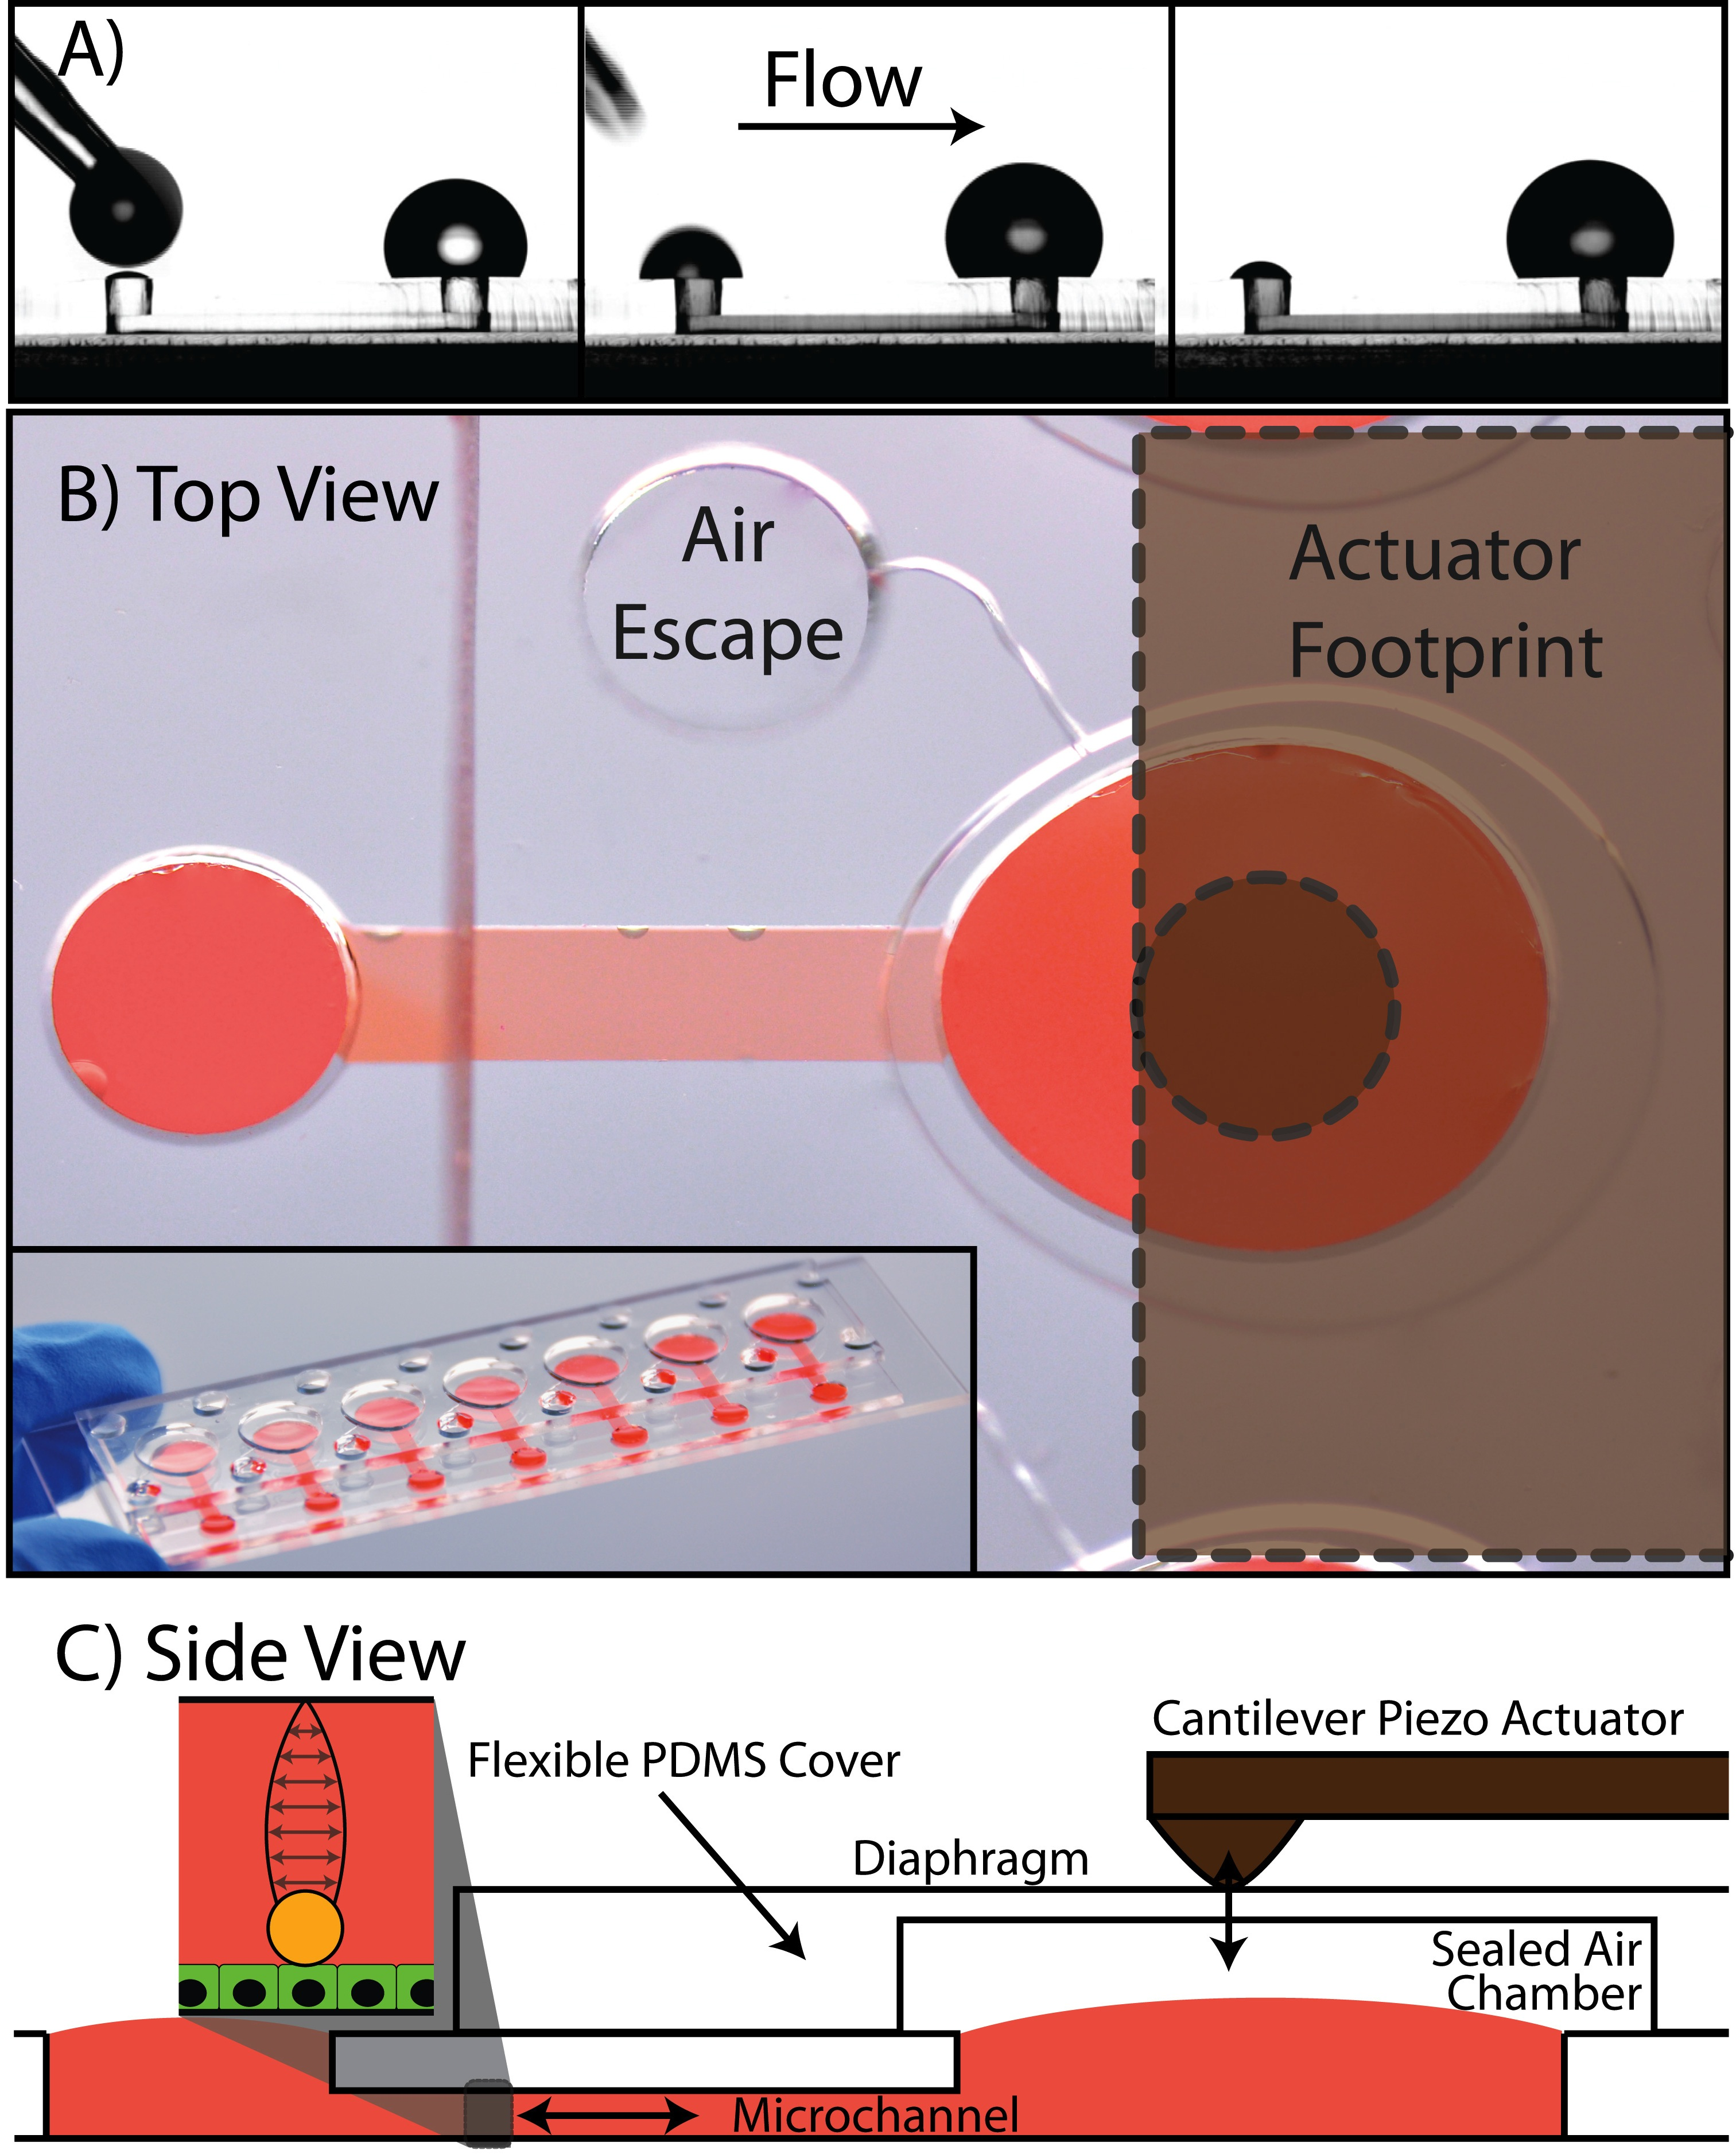
\includegraphics[width=3.5in]{OscillatoryDiagram4.jpg}
\caption{\textbf{Oscillatory flow device}. (A) Side images of passive pumping via dispensed droplets. (B) Top view of microchannel and diaphragm assembly. Inset shows 7 x 1 array of microchannels on a single microscope slide. (C) Side view of setup. Cantilever piezoelectric actuator deflects diaphragm according to applied voltage signals. At low frequency and moderate amplitude, this creates a volume change in the air cavity and displaces fluid in the channel. Oscillatory shear-stresses may be generated with this approach, allowing it to be used for various cell adhesion studies.}
\label{figure:schematic}
\end{figure}

The dimensions of the straight microchannel mimic the dimensions of a conventional parallel-plate flow chamber while the microchannel ports provide the ability to load and treat cells via pipette. The use of microfabrication techniques will allow us to rapidly explore more complex designs in the future. The footprint of the device provides a modest increase in throughput, i.e., up to seven microchannels per array during one microscope acquisition session, but perhaps more importantly, the microchannels were independently addressable. Maintaining separation ensures that each endothelial monolayer is cultured, activated, and\slash or mechanically stimulated as independent biological samples without adverse cross-talk, as is the case in many multiplexed microfluidic systems. In co-culture adhesion studies, this property has the potential for an even larger impact: the system can test limited cell samples, such as those acquired from clinical patients, as demonstrated by our use of $\sim 10^4$ cells per channel. This is a relatively small amount of cells compared to $\sim 10^6$ to $10^7$ cells typically needed for large-scale (mL) continuous flow in parallel-plate flow chambers. We envision that the system can be scaled if necessary to take even fewer cells ($10^2$ or $10^3$ cells), with only minor modifications to microchannel dimensions.

The oscillatory flow methods used here also have potential utility in other biological applications such as cardiovascular and bone mechanobiology, where oscillatory shear-stress has been implicated in important regulatory functions. Macroscale oscillatory flow systems have already been accepted into the laboratory setting while microscale oscillatory systems (and recirculatory systems in general) have also begun to appear \cite{Song:2005p157,Shao:2009p534}; however, the current design is the first oscillatory system to employ passive-pumping, thus combining the advantages of microscale approaches with simple pipette-based operation that obviate the need for tubing that inherently leads to excess dead volume.

The most innovative features of the demonstrated method are the integrated use of the piezoelectric actuator-PDMS membrane, and the development of a unique cell adhesion readout that has potential to offer new biological insights into cell adhesion phenomena. We leveraged the elastic properties of PDMS to create a sealed air chamber and diaphragm with negligible damping effects below 30 Hz and moderate amplitudes. However, oscillatory flow in a microchannel of these dimensions produces non-linear shear-stress response above 5 Hz. Above 5 Hz, the flow profile becomes non-parabolic. Above 30 Hz, the compliance of the air chamber results in significant attenuation of shear-stress. However, a property of laminar flow (steady and pulsatile) is that shear-stress at a given frequency is always linear to the pressure gradient. Clearance between the diaphragm and fluid in the port also limits actuator amplitudes. However, only 30 \textmu m of motion is required to produce the maximum shear-stress used in this study. As mentioned earlier, the microchannel ports act as reservoirs for oscillatory fluid exchange and thus limit the total volume that can be exchanged between the ports per cycle. The adhesion studies to date have been done in the low frequency regime where damping is insignificant leading to a linear relationship between frequency and shear-stress.

\subsection{Adhesion Assay via Image Differencing}

\paragraph{Measurement of Attachment \vs\ Detachment.}The use of a piezoelectric actuator enables the use of a wide variety of signal waveforms and flexible control of the shear-stress protocol. This capability allowed us to develop an 8-minute adhesion assay that samples a large range of frequencies at high resolution using a logarithmic sweep that spans two orders of magnitude (2 Hz to 100 mHz). Thus, this system provides similar resolution to that presented recently by \cite{Christophis:2010fk}. However, in contrast to Christophis \etal\ and other assays that ramp up shear-stress to detect detachment events, we have employed an inverse strategy where cells are initially prevented from adhering by starting at a relatively high shear-stress and then gradually \emph{reducing} shear-stress in order to monitor the \emph{attachment} events instead of \emph{detachment}.

\paragraph{Oscillatory \vs\ Flow-Through Methodologies}Although both oscillatory and flow-through devices can be used to study both attachment and detachment, the use of oscillatory flow fundamentally changes the readout of an attachment assay compared to flow-through devices and provides new insights into adhesion properties that have not been previously obtained. The \emph{attachment} readout of the oscillatory adhesion assay is identical to the \emph{detachment} readout reported by Christophis \etal. In the case of Christophis \etal\, the population of interest is completely defined prior to detachment, enabling them to present detachment results over a range of shear-stresses in terms of ``\% of the entire population of interest''. In doing so, they are able to directly measure the shape of the population distribution with respect to detachment shear-stress. The ability to measure the shape of the population distribution can provide important insight into the mechanisms of adhesion. In our case, the population of interest can also be defined as those cells that are initially in the field-of-view. The oscillatory nature of the flow allows us to monitor this population of interest over time for different levels of shear-stress to report the number of adhered cells as a \% of the entire population at various shear-stresses, thereby directly measuring the shape of the population distribution as well. This is different from other attachment assays that used flow-through or recirculation devices. When flow-through devices (\eg, the Christophis \etal\ device) are used in ``attachment-mode'' it becomes more difficult to define what an entire population is and makes it much more challenging to elucidate the shape of the population distribution. Thus, it is the oscillatory nature of the flow that enables a direct measurement of population distributions for attachment assays.

A previous study by Wang \etal\ used pulsing flow to study cell attachment and leveraged the ability to follow a single cell over time to examine individual attachment events; however, shear-stress in the system is uncharacterized and the readout was not extended to provide information regarding the distribution of the population \cite{Wang:2009kl}. The embodiment also differs significantly from that reported here given the use of tubes and a mechanical pumping mechanism with limited flexibility for defining complex flow patterns. Also, the study used image streams and image differencing to obtain measurements of \emph{cell motion} which were then normalized using knowledge of cell densities and suspension volumes to compare relative amounts of adhesion between two different cell populations at a given shear-stress. Here, a fully automated algorithm uses image difference information to directly measure the percent of cells adhered for an entire population over a range of shear-stresses.

\paragraph{Image Analysis: Preprocessing.}The percent of adhered cells is determined using phase-contrast microscopy. The data set for each channel consists of 41 image streams, each containing 25-170 images depending on the length of time needed to acquire 1-2 cycles of cell motion. The background is subtracted from all the images in the data set. The image used for background subtraction is determined from the first stream of images. In phase contrast using low magnification (2X), the cells appear brighter than the background. Thus, a stack projection is performed on the first stream to determine the minimum intensity for each pixel over time, removing any brighter moving objects (\ie, suspended cells) from the resulting background image. Thus, the background subtracted images in the data set are greatly enhanced to show suspended cells that were added to the channel. By using the same background image to perform all background subtraction for a given channel, any suspeded cells that adhere at a later time-point will still show up as being bright. An Otsu automatic thresholding routine is used to threshold the enhanced images to produce binary images with cells appearing white and background black. The background subtraction process produces stark contrast between the cells and background to make the automatic thresholding routine very robust. A single region of interest (ROI) is then chosen and applied to all images of the data set to restrict analysis from considering portions of the image where no cells exist and where shear-stress is uniform. Given the channel dimensions used in this study, the center 80\% of the channel width exhibits uniform shear-stress and is chosen using the ROI. All subsequent analysis is limited to this ROI.
 
\paragraph{Image Analysis: Quantifying the Percent of Adhered Cells.}Fig \ref{Chap:TumorCellAdhesion:fig:differencing} shows an idealized version of the black and white image streams that result from preprocessing and helps to describe the algorithm used to determine the percent of cells adhered to the substrate. In any given frame of a stream, there can be adhered (A) and non-adhered (NA) cells. In a different frame of the same series, non-adhered cells show up in a different location whereas adhered cells remain in the same spot. Thus, if we take the absolute difference of these two frames the non-adhered cell will show up twice whereas the adhered cell will show up once. Depending on the frames that are chosen, the impressions of the non-adhered cell may partially overlap.

\begin{figure}[!bt]
\centering
\includegraphics[width=6in]{ImageDifferencing.pdf}
\caption{\textbf{Image differencing algorithm}. $F_{n}$ refers to the $n^{th}$ frame of a time-series of images. $F_{n+\Delta n}$ refers an image taken $\Delta n$ frames after $F_{n}$. NA refers to a cell that is \underline{n}ot \underline{a}dhered where as A refers to a cell that is \underline{a}dhered.}
\label{Chap:TumorCellAdhesion:fig:differencing}
\end{figure}

If the impressions do not overlap then Eq \ref{Chap:TumorCellAdhesion:equ:percentAdhered} can be used to predict the percent of cells adhered where $F_{i}$ represents the integrated intensity of the $i^{th}$ binary image. For each stream the reference frame $F_{n}$ is chosen as the frame which exhibits the most average intensity over the course of the stream. The quantity $\left| F_{n}-F_{n+\Delta n}\right|$ is then calculated for all other images while holding $F_{n}$ constant. Partial overlap reduces the value of $\left| F_{n}-F_{n+\Delta n}\right|$ and is expected to occur less than 30\% of the time given our number of frames and minimum cell amplitudes. Therefore the top 5\% of these values are averaged to potentially reduce noise in determining a final value for the numerator of Eq \ref{Chap:TumorCellAdhesion:equ:percentAdhered}. This number is proportional to twice the number of non-adhered cells whereas $F_{n}$ is proportional to the number of total cells, thus arriving at Eq \ref{Chap:TumorCellAdhesion:equ:percentAdhered} for the percent of adhered cells. This process is repeated for each of 41 streams in the data set for each channel to produce a plot of `\% of Population Adhered' \vs\ `Shear-Stress'. It is possible that if oscillation and image acquisition were synchronized, image streams would no longer be necessary as a good choice for $F_{n}$ and $F_{n+\Delta N}$ can be predicted based on the sinusoidal nature of the oscillation.

\begin{equation}
\textrm{\% of Pop. Adhered} = 1 - \frac{\left| F_{n}-F_{n+\Delta n}\right|}{2 \, F_{n}}
\label{Chap:TumorCellAdhesion:equ:percentAdhered}
\end{equation}

\paragraph{Batch Processing.}The image filtering and analysis is completely automated using custom software called Je'Xperiment, developed by Jay Warrick and Erwin Berthier at the University of Wisconsin Madison. The software is used to database the images and perform batch processing of the custom algorithm. One array of 7 channels produces approximately 10-15 gigabytes of data. The primary time constraint of the analysis is thus the time it takes to read and write the images to a hard drive or server ($\sim$ 5 hours total). However, Je'Xperiment allows one to obtain results with less than 10 minutes of time actually invested by the user at the computer workstation.

\paragraph{Interpretation of Results.}Fig \ref{Chap:TumorCellAdhesion:fig:logNorm} illustrates the shape of the resulting adhesion plot and the log-normal cumulative distribution function (LNcdf) used to fit the data. The LNcdf (Eq \ref{Chap:TumorCellAdhesion:equ:LNcdf}) has two parameters, $\mu$ and $\sigma$, which are obtained from the curve fit. The quantity $e^{\mu}$ represents the median shear-stress of the population, $\tau_{50}$, whereas $\sigma$ indicates the spread, measured in orders of magnitude, of the data surrounding the median. This interpretation is different than a normal distribution where $\sigma$ gives an indication of absolute spread about the mean.

\begin{figure}[!t]
\centering
\includegraphics[width=3.5in]{TheoryPlot.pdf}
\caption{\textbf{Log-normal cumulative distribution function}.}
\label{Chap:TumorCellAdhesion:fig:logNorm}
\end{figure}

\begin{equation}
\textrm{LNcdf($x$,$\mu$,$\sigma$)} = \frac{1}{2} + \frac{1}{2}\textrm{erf}\left[ \frac{\ln{x} - \mu}{\sqrt{2 \sigma^{2}}}\right] 
\label{Chap:TumorCellAdhesion:equ:LNcdf}
\end{equation}

Interpretation of changes in the median are fairly straight forward but changes in $\sigma$ are less intuitive. For example, assume there is a cell type and a substrate that interact via one type of molecule with a median shear-stress of 1 Pa and has a $\sigma$ of 1 indicating that 97.89\% of all cells in the population adhere at a shear-stress between 0.1 and 10 Pa. In this idealized scenario, if the substrate is changed such that only 1/10$^{th}$ the original amount of adhesion ligand is presented to the cells, one would expect the median shear-stress to drop to roughly 0.1 Pa given that the number of anchor points per cell is lowered accordingly. Since each portion of the population would fall under this argument, shear-stress data would be predicted to simply shift while keeping $\sigma$ the same. That is to say, the new median shear-stress would be 0.1 Pa with 97.89\% of the population falling between 0.01 and 1 Pa.

On the other hand, what if the median does not change and $\sigma$ does? Given $\sigma$ is a measure of the heterogeneity of the interaction between the cells and substrate, a change in $\sigma$ indicates that the type of mechanism mediating adhesion (\ie\ the involvement of specific molecules or physical forces) has changed or has become more or less heterogeneous. However, it is more likely that multiple molecules or mechanisms mediate adhesion and contribute to an overall perceived heterogeneity. In this situation, if the influence of one of those contributing mechanisms were to be heightened, the value of $\sigma$ would change as well. If a single population has two dominant mechanisms of adhesion, it would result in the multiplication of two characteristic LNcdfs. On the other hand, if there are \emph{two} distinct populations, the result would be the renormalized addition of the two characteristic LNcdfs.

Thus, changes in $\sigma$ are associated with changes in the heterogeneity of the underlying mechanism, whereas changes in the median indicate changes in the strength or number of the interactions.

\subsection{Cancer cell adhesion}
Having defined the oscillatory attachment assay methodology, readout, and method of data interpretation; biological experiments are performed to characterize the sensitivity and repeatability of the assay for detecting physiologically relevant changes in adhesion interactions. We tested adhesion of three established cell lines derived from distinct types of cancer, including prostate (PC3-MM2), breast (MDA-MB231), and multiple myeloma (RPMI8226).  Studies on the adhesiveness, invasiveness and metastatic potential of these cell lines have shown that PC3-MM2 cells are particularly invasive among PC3 family of sublines \cite{Daja:2003rr}, and that PC3 sublines are highly variable in adhesiveness \cite{Dimitroff:2004bh}. MDA-MB231 cells are also highly invasive among breast cancer cell lines \cite{TOZEREN:1995wd,Lee:2003kx}, but are known to adhere to activated endothelium only in the absence of shear-stress $> 0.5$ dyn/cm$^2$ \cite{TOZEREN:1995wd}. In contrast to prostate and breast cancers, the adhesiveness and invasiveness of cells of multiple myeloma (MM) origin has been studied to a much lesser extent. Reports of MM cell adhesion that are available seem to suggest that adhesion to (bone marrow) endothelium is mediated by various molecules other than E-selectin \cite{Okada:1995ys,Broek:2008p301,Katz:2010uq}. Thus, we expected that PC3-MM2 and MDA-MB231 cells would exhibit more adhesive phenotypes, while RPMI8226 would likely show less adhesion to the endothelial monolayers.

We performed independent LNcdf curve fits for each condition, extracted the fitted $\tau_{50}$ and $\sigma$ values and compared results between activated and non-activated endothelium as well as across the different cell types. Fig \ref{Chap:TumorCellAdheison:fig:examples} shows examples of data and LNcdf fits for each cell type on activated and non-activated endothelium.

\begin{figure}[ht] %DONE
\centering
\begin{tabular}{cc}
A) PC3-MM2 & B) RPMI8226 \cr
\includegraphics[width=2.5in]{ExamplePC3.pdf} &\includegraphics[width=2.5in]{ExampleRPMI.pdf} \cr
C) MDA-231 & \cr
\includegraphics[width=2.5in]{ExampleMDA.pdf}
\end{tabular}
\caption{\textbf{Example adhesion curves for each condition}. Each pair of curves represents a adhesion measured in two channels on the same day. (blue) Non-activated endothelium. (red) Activated endothelium. }
\label{Chap:TumorCellAdheison:fig:examples}
\end{figure}

We observed statistically significant increases in $\tau_{50}$ (the critical shear-stress) between activated and non-activated endothelial surfaces for all cell types, including, surprisingly, RPMI8226 cells (Figure \ref{Chap:TumorCellAdhesion:fig:summaryGraphs}A). Comparing non-activated endothelium cases alone, both MDA-MB231 and PC3-MM2 cells exhibited significantly higher values of $\tau_{50}$ than RPMI8226 cells; this was also true for the activated endothelium cases alone, where MDA-MB231 and PC3-MM2 cells had higher $\tau_{50}$ than RPMI8226 cells (Figure \ref{Chap:TumorCellAdhesion:fig:summaryGraphs}A). Interestingly, when the \emph{ratio} between activated and non-activated $\tau_{50}$ values were calculated and compared, no difference was found between cell types (Figure \ref{Chap:TumorCellAdhesion:fig:summaryGraphs}B), suggesting that the effect of IL-1$\beta$ induction on adhesion was consistent across cell types. Thus, MDA-MB231 and PC3-MM2 cells were likely more adhesive than RPMI8226 cells because of intrinsic differences in cell surface properties, which were amplified for all cell types in the presence of E-selectin. This appeared to be consistent with the literature cited above.

\begin{figure}[!tb] %DONE
\centering
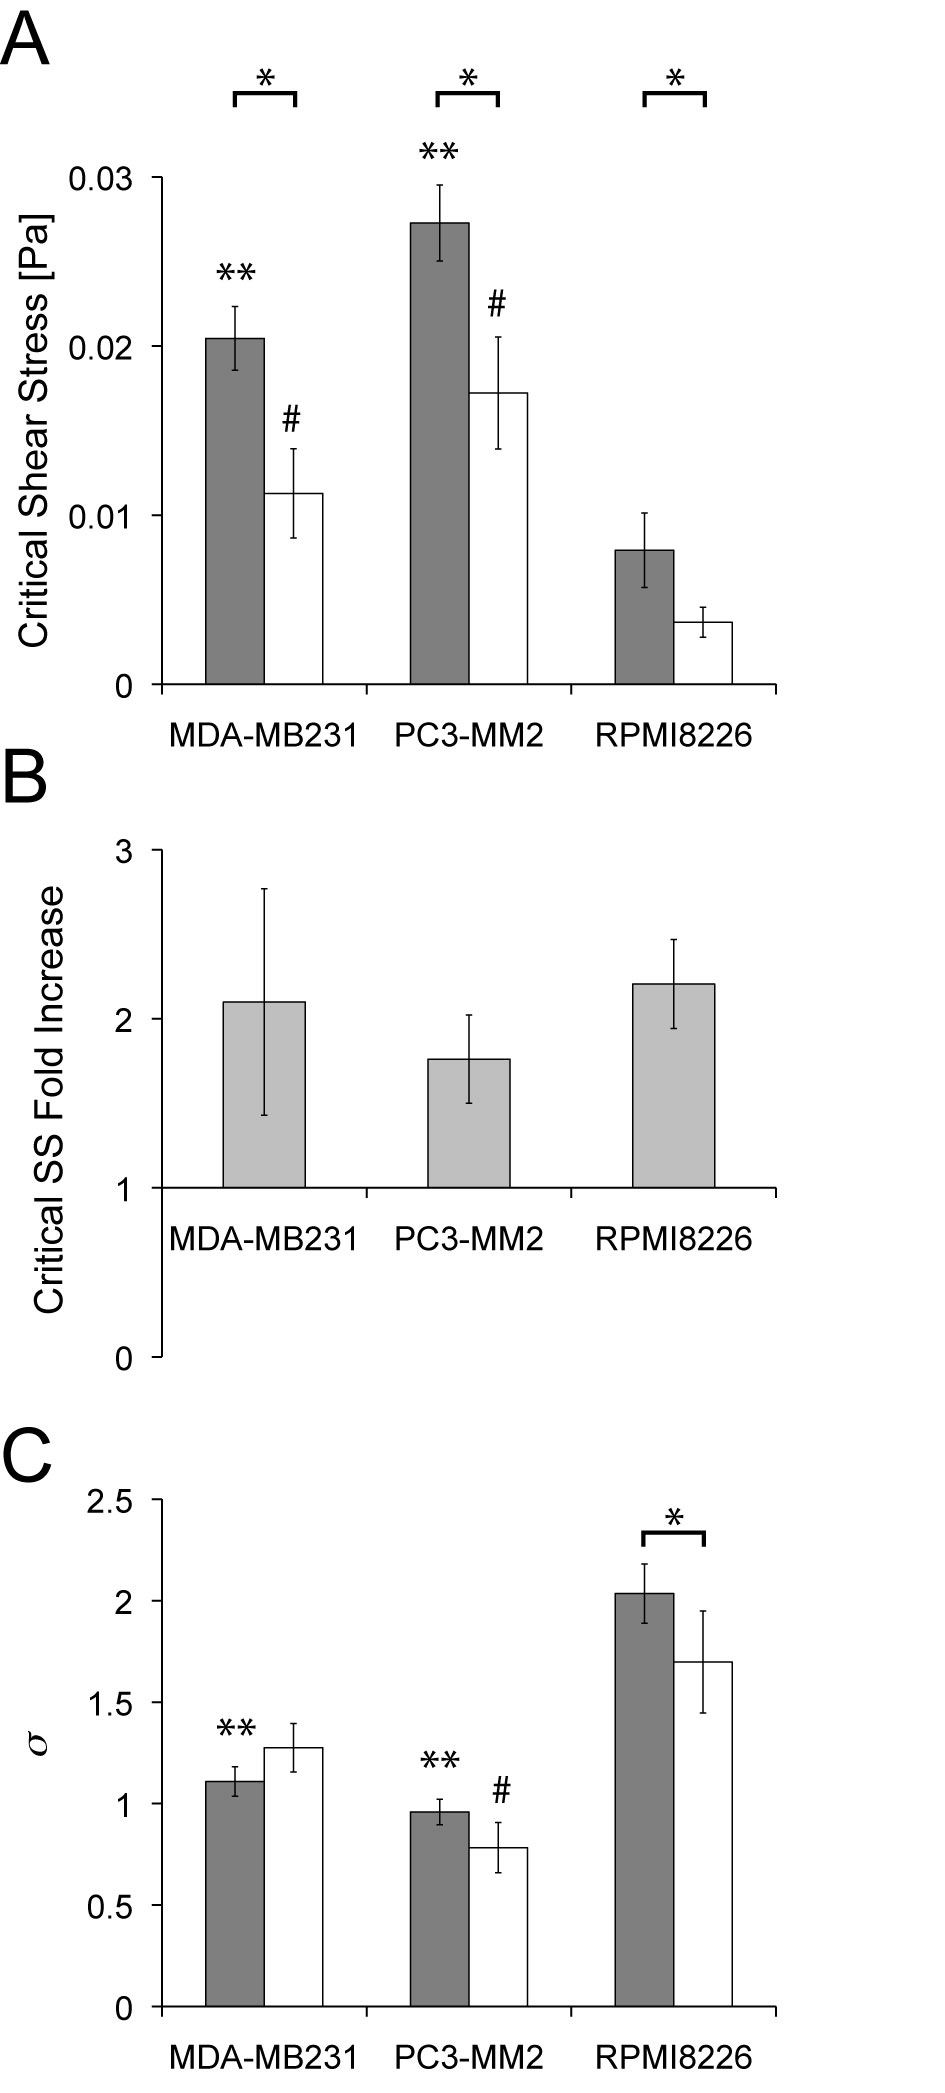
\includegraphics[height=6in]{Figure_FinalGraphs.jpg}
\caption{\textbf{Comparison of adhesion to a HUVEC monolayer}. (A) Average critical shear-stress on activated (gray bars) and non-activated (white bars) endothelium. (B) Average fold increase in critical shear-stress. (C) Average $\sigma$ of lognormal distribution on activated (gray bars) and non-activated (white bars) endothelium. $\ast: P < 0.05$ for combined block multiple experiments between activated and non-activated endothelium for given cell type. $\ast\ast: P < 0.05$ compared to RPMI8226 on activated endothelium.  $\#: P < 0.05$ compared to RPMI8226 non-activated endothelium.}
\label{Chap:TumorCellAdhesion:fig:summaryGraphs}
\end{figure}

Fitted values of $\sigma$ were also compared between non-activated and activated endothelium groups and  across cell types. No statistically significant differences were found between activated and non-activated endothelium conditions for comparisons within each cell type (Figure \ref{Chap:TumorCellAdhesion:fig:summaryGraphs}C). However, $\sigma$ values for RPMI8226 cells were significantly higher than those for PC3-MM2 and MDA-MB231 for both activated and non-activated endothelium groups. These data suggested that $\sigma$, which represents the heterogeneity in cell adhesion of the population, was not influenced by endothelial activation, but only by intrinsic differences between cells. 

Collectively, the pair of fitted parameters $\tau_{50}$ and $\sigma$ have revealed expected yet nevertheless interesting similarities and differences between the cancer cell types, which can be interpreted as follows. No difference in the heterogeneity of the metastatic breast and prostate cancer cell line adhesion could be observed and this heterogeneity did not change significantly upon activation of the endothelium. That is to say, although endothelial activation enhanced adhesion for these two cell types, the level of enhancement was consistent across all individual cells within the population (i.e., no change in spread in the LNcdf was observed), and consistent across cell types (\ie, no significant change in the fold-increase of $\tau_{50}$ was observed either). RPMI8226 cells were similarly affected by endothelial activation, but in comparison to PC3-MM2 and MDA-MB231 cells, RPMI8226 cells were much less adherent and displayed much more heterogeneity in the population. This heterogeneity is potentially related to its low adherence, since loose adhesion from non-specific interactions is likely to yield low $\tau_{50}$ and high $\sigma$. 

\section{Conclusion}
A novel approach for examining cell attachment has been presented that integrates a unique method for producing oscillatory flow, high resolution sweep of shear-stress, fully automated image analysis algorithm, and comprehensive examination of population heterogeneity. The sensitivity and repeatability of the method was validated by confirming an increase in adhesion of three different tumor cell lines representing 3 different cancers to a HUVEC monolayer upon activation of the monolayer using IL-1$\beta$. Unique insight into population heterogeneity was enabled by the use of oscillatory flow. The use of oscillatory flow also enabled the use of passive-pumping to allow samples to be loaded and treated using a pipette. Thus, the platform enables complete separation of microchannels to ensure independence of each data point acquired in the array. Taken together, the method presented here offers new insight into cell adhesion, represents a significant advance to the study of cell attachment, and has the potential to advance our understanding of adhesion in areas such as cancer metastasis, inflammation, and regenerative medicine.

\section{Materials and Methods}

\subsection{Cell Culture}

Human umbilical vein endothelial cells (HUVECs) were purchased from Lonza (Walkersville, MD), and regularly cultured on tissue culture-treated flasks pre-coated with 1.5 $\mu$g/cm$^2$ of bovine plasma fibronectin (FN) (Sigma-Aldrich, St. Louis, MO). HUVECs were maintained in EGM BulletKit media (CC-3124, Lonza) consisting of EBM-2 basal medium supplemented with 2\% fetal bovine serum (FBS), bovine brain extract with heparin, hEGF, hydrocortisone, and gentamicin/Amphotericin B. HUVECs were fed every other day, passaged every 3-4 days at 90\% confluence, and only passages 4-6 were used in microchannel experiments. 

To prepare HUVEC monolayers for adhesion tests, microchannels were first primed with 30 $\mu$L PBS followed by 20 $\mu$L FN at 100 $\mu$g/mL concentration. Microchannels were incubated at 37 deg C for 1 h in humidified trays to allow FN adsorption to the microchannel walls. After incubation, FN was replaced twice with 40 $\mu$L HUVEC media further supplemented with 10 mM HEPES. HUVECs were seeded at 3000 cells/$\mu$L $\times$ 6 $\mu$L per microchannel, and allowed to adhere and culture overnight (12 h). HUVEC microscale cultures were either used on the same day for adhesion tests if confluent, or maintained for an additional day to reach full confluence. Activated HUVEC monolayers in microchannels were induced with 10 $\mu$g/mL interleukin-1$\beta$ (IL-1$\beta$) for 4 h before adhesion tests.

Three different human cancer cell lines were used in adhesion tests to compare adhesion strengths on activated versus non-activated endothelium. MDA-MB231 cells (mammary gland epithelial) were maintained in DMEM with 4.5 g/L glucose supplemented with 10\% FBS and 1\% penicillin/streptomycin (P/S). PC-3 MM2 cells (metastatic prostate) were maintained in RPMI1640 with L-glutamine, 10\% FBS, 1\% penicillin/streptomycin (P/S), and 10 mM HEPES. RPMI8226 cells (multiple myeloma in bone marrow) were maintained in DMEM with 4.5 g/L glucose supplemented with 10\% FBS, 1\% P/S, and 10 mM HEPES.  MDA-MB231 and PC3-MM2 cells were fed every other day and passaged every 3-4 days depending on confluence. RPMI8226 cells were passaged every 3 days. All cell lines were resuspended at 1000-1500 cells/$\mu$L, and 7.5 $\mu$L of cell suspension was dispensed into each microchannel. Thus, each microchannel contained approx. 7,500 to 12,000 cells.

\subsection{Immunostaining and HUVEC activation}

Immunostaining was performed to verify upregulation of E-selectin upon activation using IL-1$\beta$. Fig \ref{Chap:TumorCellAdhesion:fig:staining} shows that E-selectin upregulation was robust for all concentrations tested while the control showed basal levels. Acquisition parameters were identical and images were treated uniformly.

\begin{figure}[!ht]
\centering
\includegraphics[width=3.5in]{StainingImages.pdf}
\caption{\textbf{HUVEC staining for E-selectin}. Concentration of IL-1$\beta$ is indicated in the corner of each image.}
\label{Chap:TumorCellAdhesion:fig:staining}
\end{figure}


\subsection{Image Capture and Analysis}

Prior to data acquisition, a calibration procedure described in Chapter \ref{Chap:Oscillator} was used to measure the initial shear stress of the system at 140 mV piezo voltage and 2 Hz sinusoidal oscillation frequency. The actuator was perturbed by gentle tapping to redistribute cells within the field of view that moved due to the calibration procedure. After waiting 30 seconds for cells to settle, the acquisition protocol was started.

Data acquisition consists of 41 stream acquisitions. The first 5 are to be acquired at 2 Hz. At the start of the sixth stream, a descending log frequency sweep is begun that lasts for 500 s and ends at 0.1 Hz. The first six datapoints obtained at a frequency of 2 Hz are used to normalize each curve. The average of those six measurements is forced to a value of one resulting in a proportional adjustment of all other values.

MetaMorph was used to acquire the image streams at specified intervals of time using the journaling capability of the software. The software also allows for the logging of times. The time at the beginning of each image stream is recorded to allow back-calculation of the frequency. This is helps improve accuracy because MetaMorph is not able to perform each stream acquisition at precisely the same time for each channel due to variability in data read-write times. The number of frames per stream was chosen to ensure capture of 1-2 cycles of fluid\slash cell motion and ranged from 25 to 170. Variable numbers of frames were used to limit the amount of data.

Images were acquired at 2X with a binning of 2 $\times$ 2 and an exposure time of 15 ms. The Ph1/PhC phase rings were used to provide maximal contrast (\ie, dark background and bright cells).

\subsection{Statistical Analyses}

\paragraph{Effects of activation.} Median $\tau_{50}$ and standard deviation $\sigma$ were determined from the lognormal curve fits for each condition (HUVEC activation and cell type), and statistically compared using nonparametric tests. First, to determine whether activation of HUVEC monolayers via IL-1beta induction had an effect on cell adhesion for each cell type, we used a combined Wilcoxon rank sum approach proposed by Lehmann (1998) for handling the complete data set consisting of multiple experiments with varying sample sizes. This required that we group our data into blocks for the separate experiments, with each block consisting of $m$ activated and $n$ non-activated monolayers.

\paragraph{Differences between cell type.} Independent Kruskal-Wallis tests were used to determine whether differences in $\tau_{50}$ and $\sigma$ were present across cell types for both the activated and non-activated monolayers. We further normalized $tau_{50}$ by defining the ratio or ``fold-increase'' of activated to non-activated adhesion, and performed Kruskal-Wallis analysis on normalized $tau_{50}$. All Kruskal-Wallis tests were performed on values averaged across samples in the same experiment.

When Kruskal-Wallis tests revealed significant differences in the data, post hoc multiple comparison tests were performed via independent Wilcoxon rank-sum tests, with and without Bonferroni correction, between separate pairs of cell types to determine which cell types differed from the others. 

\paragraph{Outliers.} Coefficients of determination ($R^{2}$) were calculated for each curve fit, and it was found that $R^{2}$ = 0.94 +/- 0.06 for the fifty experiments we conducted. One outlier was detected ($R^{2}$ = 0.60), and removal of the outlier resulted in $R^{2}$ = 0.95 +/- 0.04. The above statistical tests were done with both inclusion and exclusion of the outlier, and it was found that the main conclusions were not affected by the presence of the outlier.




